\Aufgabe[e]{Integral \"uber Kreisring}{
Gegeben sei ein Kreisring
$$
R = \left\{ \vec x \in \mathbb{R}^2 | 1 \leq \| \vec x \| \leq 2 \right\}
$$
Weiterhin sei die Funktion
$$
f(x,y) = \operatorname{e}^{x^2+y^2} y^2
$$
gegeben.
\begin{abc}
\item Skizzieren sie den Integrationsbereich $R$.
\item Bestimmen Sie das Integral $I = \int_R f(x,y) \mathrm{d} (x,y).$
\end{abc}

}

\Loesung{
\begin{abc}
\item
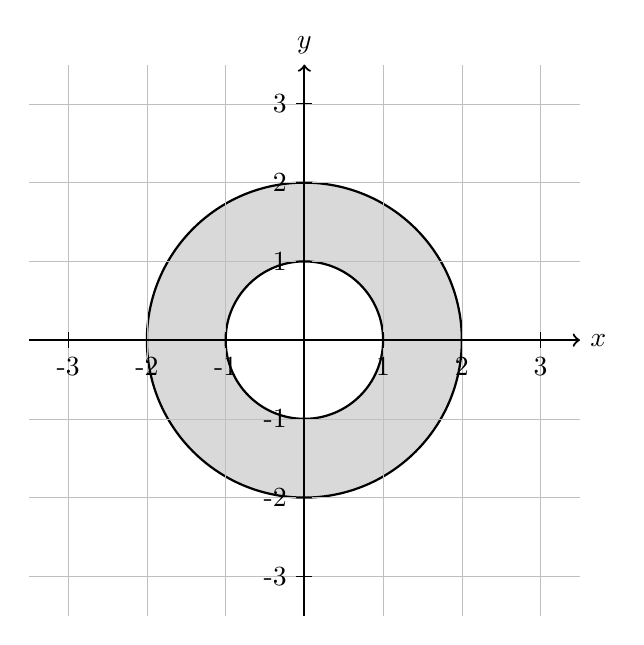
\begin{tikzpicture}
  % Kreisring im Hintergrund
  \begin{scope}
    \fill[gray!30] (0,0) circle (2);
    \fill[white] (0,0) circle (1);
    \draw[thick] (0,0) circle (1);
    \draw[thick] (0,0) circle (2);
  \end{scope}

  % Gitter und Achsen im Vordergrund
  \draw[step=1cm,gray!50,very thin] (-3.5,-3.5) grid (3.5,3.5);
  \draw[->, thick] (-3.5,0) -- (3.5,0) node[right] {$x$};
  \draw[->, thick] (0,-3.5) -- (0,3.5) node[above] {$y$};

  % Achsenbeschriftungen
  \foreach \x in {-3,-2,-1,1,2,3}
    \draw (\x,0.1) -- (\x,-0.1) node[below] {\x};
  \foreach \y in {-3,-2,-1,1,2,3}
    \draw (0.1,\y) -- (-0.1,\y) node[left] {\y};
\end{tikzpicture}


\item
Wir stellen das Integral in Polarkoordinaten dar.
$$
x = r \cos(\varphi) , \quad y = r \sin(\varphi)
$$
Es gilt dann:
\begin{align*}
I &= \int_1^2 \int_0^{2\pi} \operatorname{e}^{r^2} r^2 \sin^2(\varphi) \cdot r \mathrm{d} \varphi \mathrm{d} r \\
&= \int_1^2 \int_0^{2\pi} \operatorname{e}^{r^2} r^3 \sin^2(\varphi) \mathrm{d} \varphi \mathrm{d} r \\
&= \int_1^2 \operatorname{e}^{r^2} r^3 (\frac{1}{2}(\varphi -\sin(\varphi)\cos(\varphi))\Big |_0^{2\pi}\mathrm{d} r \\
&= \pi \int_1^2 \operatorname{e}^{r^2} r^3 \mathrm{d} r \\
\end{align*}
Um dieses Integral zu l\"osen wird eine Substitution mit $u=r^2$ und $\mathrm{d}u = 2r \mathrm{d}r$ und anschlie\ss end eine partielle Integration durchgef\"uhrt:
\begin{align*}
I &= \pi \int_1^4 \operatorname{e}^u u  \cdot \frac{1}{2} \mathrm{d} u \\
&= \frac{\pi}{2} \left(\operatorname{e}^u u \Big |_1^4 - \int_1^4 \operatorname{e}^u \mathrm{d} r\right)\\
&=\frac{\pi}{2} \left(\operatorname{e}^u u \Big |_1^4 - \operatorname{e}^u \Big |_1^4\right)\\
&=\frac{3\operatorname{e}^4 \pi}{2}
\end{align*}
\end{abc}
}

\ErgebnisC{AnalysIntgPola001}{
$I= \frac{3\operatorname{e}^4 \pi}{2}$
}
